\documentclass[12pt,a4paper]{article}
\usepackage{amsmath}
\usepackage{graphicx}
\usepackage{geometry}
\usepackage{float}
\geometry{left=2cm,right=2cm,top=2.5cm,bottom=2.5cm}

\title{\textbf{Kinematic and Singularity Analysis Report \\ with Explicit Matrix Operations}}
\author{Automated Generation System}
\date{\today}

\begin{document}
\maketitle

\section{Mathematical Formulation}
The closed-loop spatial kinematic constraint is given by:
\begin{equation}
    T_1(q_1) T_2(q_2) T_3(q_3) T_4(q_4) T_5(q_5) T_6(q_6) T_7(q_7) = I
\end{equation}
The velocity constraint yields $J_p \dot{\mathbf{q}}_p = - J_a \dot{q}_1$, where $J_p$ is the $6 \times 6$ passive Jacobian matrix obtained by removing the column corresponding to the driving joint $J_1$.

\section{Example Matrix Calculation at $q_1 = 0^\circ$}
To demonstrate the calculation process, we extract the system matrices at the initial driving configuration ($q_1 = 0$ rad). The solved full joint configuration (in radians) is:
\begin{equation}
    \mathbf{q} = \begin{bmatrix} 0.0000 \\ -0.0234 \\ -0.0002 \\ 0.0469 \\ 0.0003 \\ 0.0234 \\ -0.0005 \end{bmatrix}
\end{equation}

Based on this configuration, the full $6 \times 7$ Jacobian matrix $J$ is evaluated as:
\begin{equation}
    \resizebox{0.95\textwidth}{!}{$ J = \begin{bmatrix}
  0.000 & 0.000 & 0.000 & 2.499 & 0.059 & -2.500 & -0.000 \\
  0.000 & -1.000 & -0.000 & 2.999 & 0.000 & 1.998 & -0.000 \\
  -0.000 & 0.000 & -3.000 & -0.059 & -0.500 & -0.059 & -2.000 \\
  0.000 & 0.000 & 0.000 & -0.023 & 0.000 & -0.023 & -0.001 \\
  0.000 & 0.000 & -1.000 & -0.000 & -1.000 & -0.000 & 1.000 \\
  1.000 & 1.000 & 0.000 & -1.000 & -0.000 & 1.000 & -0.000
\end{bmatrix} $}
\end{equation}

By extracting the columns corresponding to the passive joints, we form the passive Jacobian $J_p \in \mathbb{R}^{6 \times 6}$:
\begin{equation}
    \resizebox{0.85\textwidth}{!}{$ J_p = \begin{bmatrix}
  0.000 & 0.000 & 2.499 & 0.059 & -2.500 & -0.000 \\
  -1.000 & -0.000 & 2.999 & 0.000 & 1.998 & -0.000 \\
  0.000 & -3.000 & -0.059 & -0.500 & -0.059 & -2.000 \\
  0.000 & 0.000 & -0.023 & 0.000 & -0.023 & -0.001 \\
  0.000 & -1.000 & -0.000 & -1.000 & -0.000 & 1.000 \\
  1.000 & 0.000 & -1.000 & -0.000 & 1.000 & -0.000
\end{bmatrix} $}
\end{equation}

Applying Singular Value Decomposition (SVD) on $J_p = U \Sigma V^T$, the decomposition yields the left singular vectors $U$:
\begin{equation}
    \resizebox{0.85\textwidth}{!}{$ U = \begin{bmatrix}
  0.665 & 0.090 & 0.637 & -0.002 & 0.379 & 0.002 \\
  0.671 & -0.026 & -0.738 & 0.006 & 0.068 & 0.009 \\
  -0.054 & 0.985 & -0.083 & 0.142 & 0.001 & -0.000 \\
  -0.005 & 0.000 & 0.008 & 0.000 & -0.010 & 1.000 \\
  -0.008 & 0.141 & -0.020 & -0.990 & 0.009 & 0.000 \\
  -0.323 & -0.038 & -0.207 & 0.010 & 0.923 & 0.009
\end{bmatrix} $}
\end{equation}

The singular values matrix $\Sigma$ (diagonal):
\begin{equation}
    \resizebox{0.85\textwidth}{!}{$ \Sigma = \begin{bmatrix}
  4.178 & 0.000 & 0.000 & 0.000 & 0.000 & 0.000 \\
  0.000 & 3.671 & 0.000 & 0.000 & 0.000 & 0.000 \\
  0.000 & 0.000 & 3.352 & 0.000 & 0.000 & 0.000 \\
  0.000 & 0.000 & 0.000 & 1.669 & 0.000 & 0.000 \\
  0.000 & 0.000 & 0.000 & 0.000 & 0.892 & 0.000 \\
  0.000 & 0.000 & 0.000 & 0.000 & 0.000 & 0.000
\end{bmatrix} $}
\end{equation}

And the transposed right singular vectors matrix $V^T$ (representing joint couplings):
\begin{equation}
    \resizebox{0.85\textwidth}{!}{$ V^T = \begin{bmatrix}
  -0.238 & 0.041 & 0.958 & 0.018 & -0.154 & 0.024 \\
  -0.003 & -0.843 & 0.035 & -0.171 & -0.102 & -0.498 \\
  0.158 & 0.080 & -0.122 & 0.029 & -0.975 & 0.044 \\
  0.002 & 0.338 & -0.003 & 0.551 & 0.011 & -0.763 \\
  0.958 & -0.015 & 0.258 & 0.014 & 0.123 & 0.007 \\
  -0.019 & -0.408 & -0.011 & 0.816 & 0.008 & 0.408
\end{bmatrix} $}
\end{equation}

\section{Analysis Results \& Curve Fitting}
\begin{figure}[H]
    \centering
    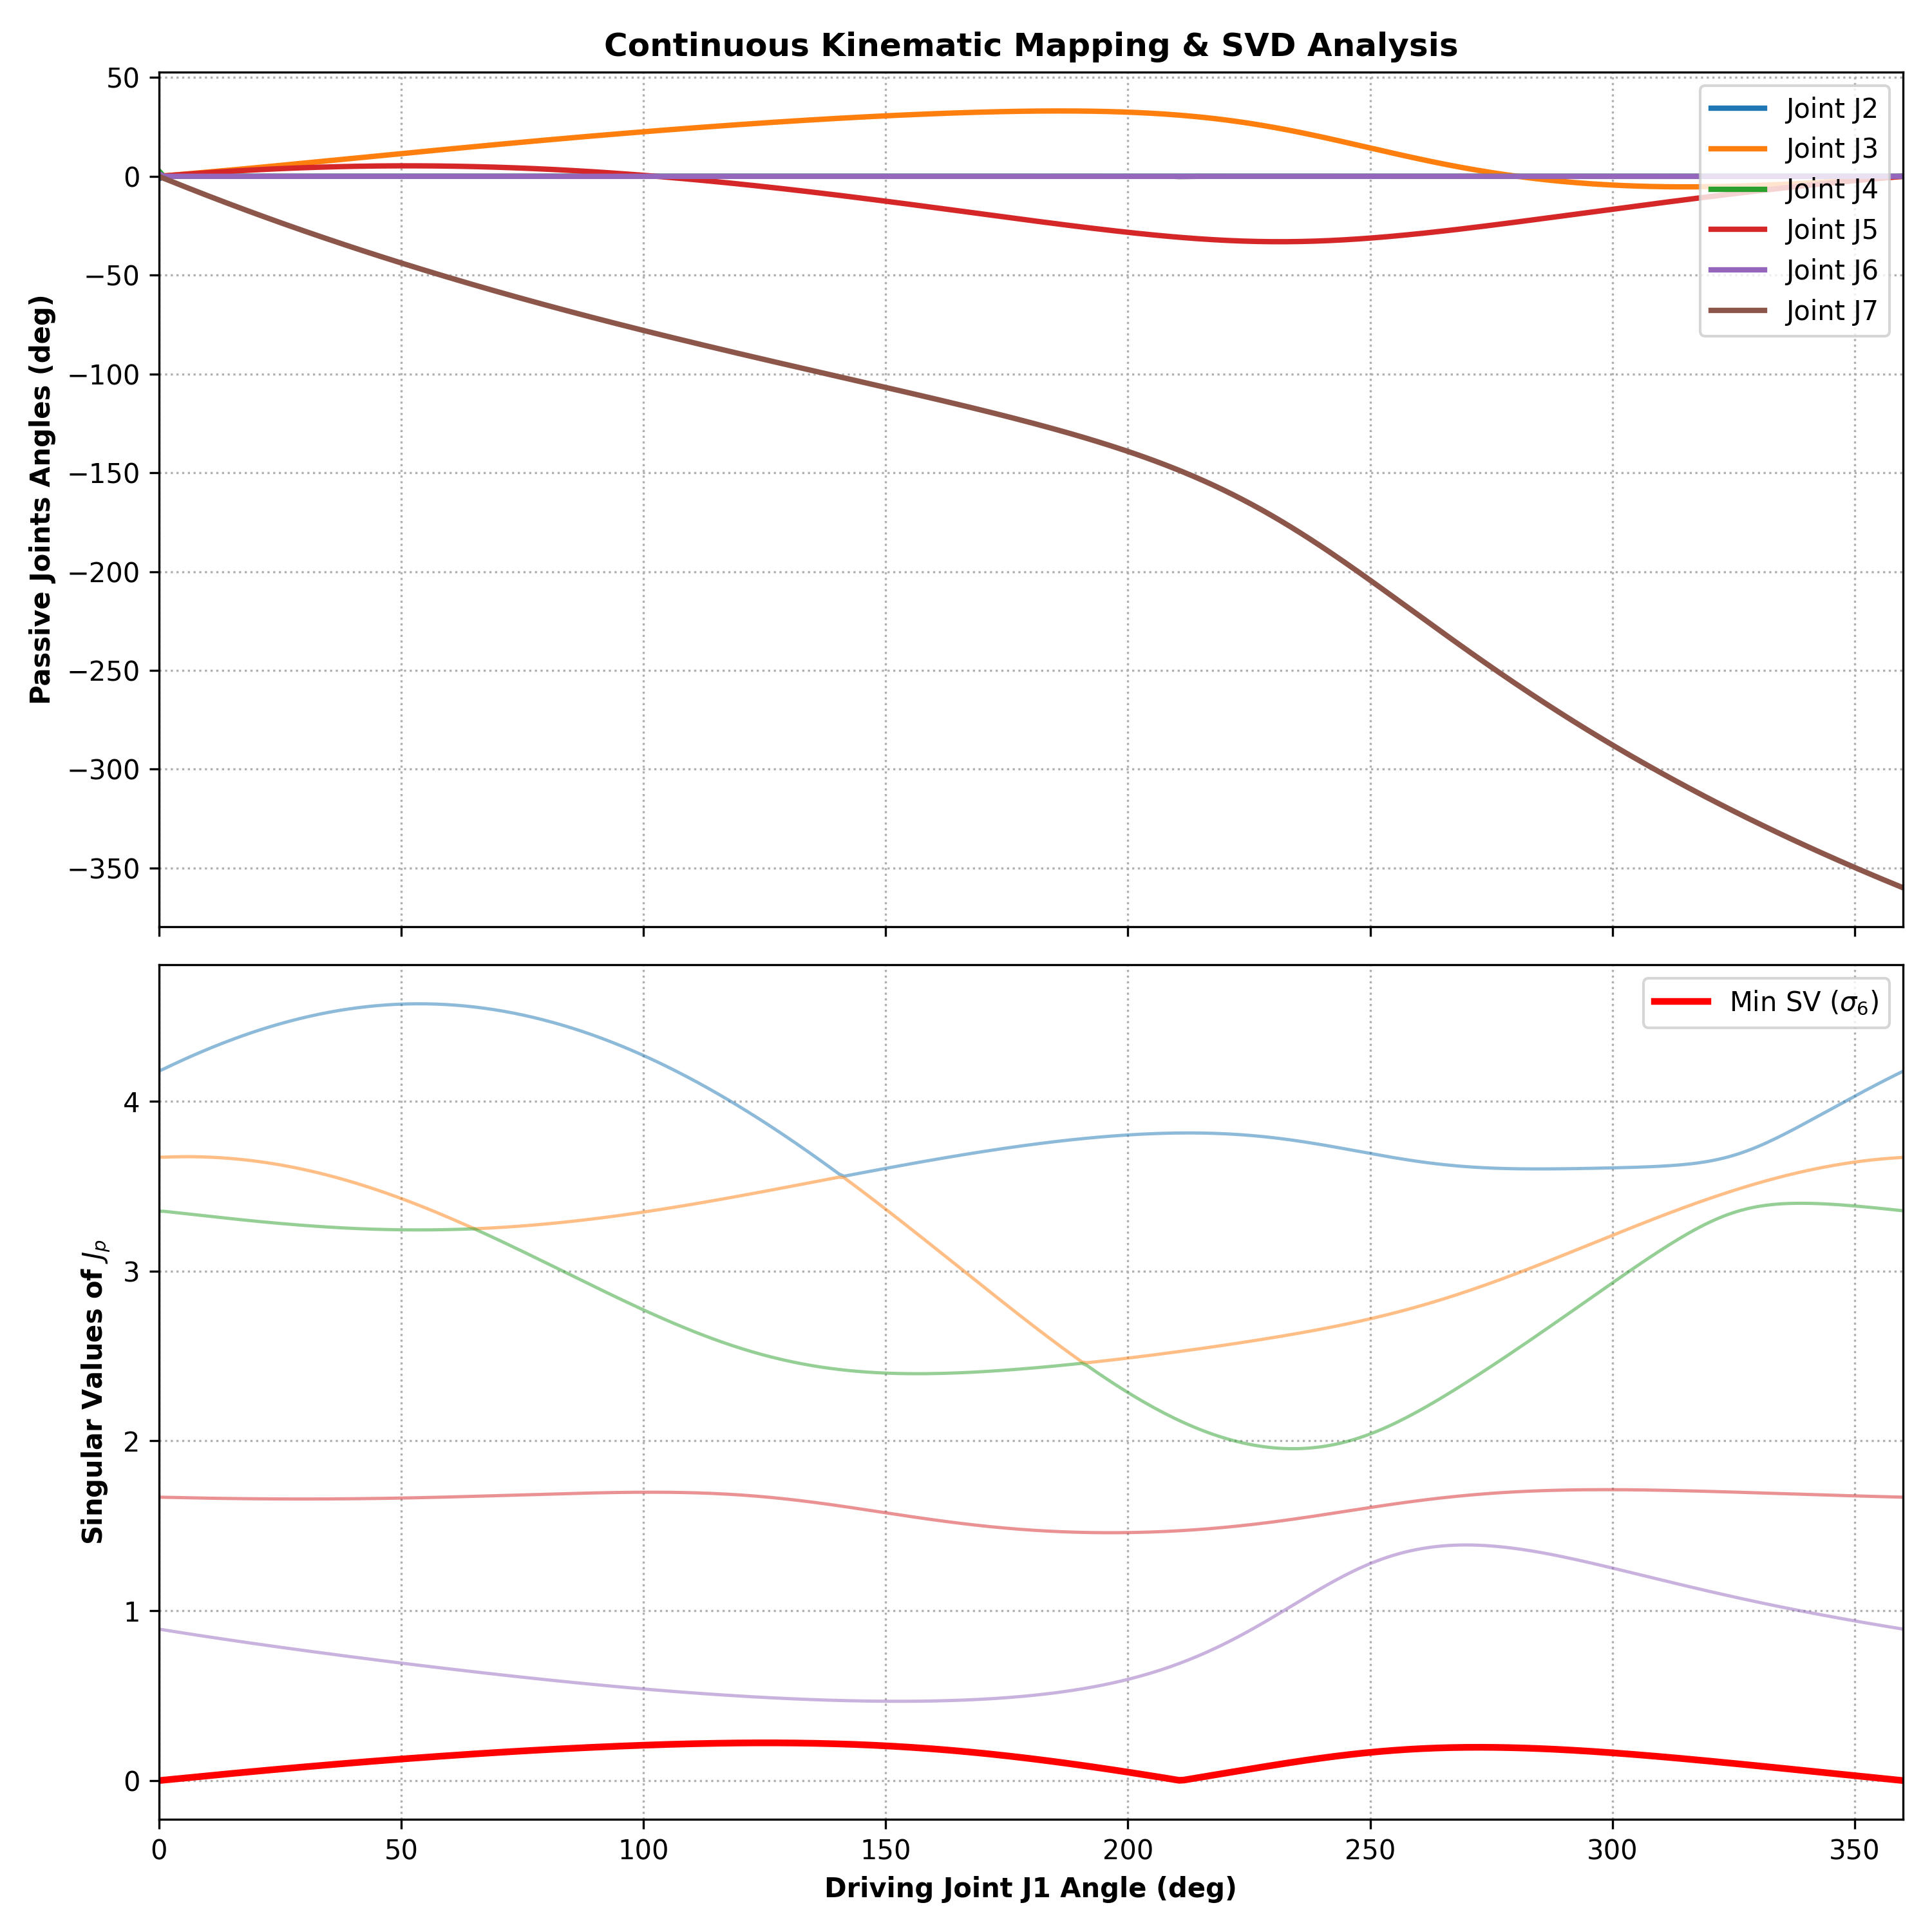
\includegraphics[width=0.9\textwidth]{j1_analysis_plot.png}
    \caption{Kinematic mapping and singular value evolution driven by $J_1$.}
\end{figure}

The Fourier series expressions for the passive joints are:
\begin{itemize}
\item \textbf{Joint J2:} \\ $Q_{J2}(x) = -0.004 -0.008\cos(x) -0.000\sin(x) -0.008\cos(2x) +0.001\sin(2x) -0.008\cos(3x) -0.001\sin(3x)$
\item \textbf{Joint J3:} \\ $Q_{J3}(x) = +14.740 -17.160\cos(x) +7.200\sin(x) +2.093\cos(2x) +3.424\sin(2x) +0.617\cos(3x) -0.949\sin(3x)$
\item \textbf{Joint J4:} \\ $Q_{J4}(x) = +0.007 +0.017\cos(x) +0.001\sin(x) +0.015\cos(2x) -0.001\sin(2x) +0.016\cos(3x) +0.001\sin(3x)$
\item \textbf{Joint J5:} \\ $Q_{J5}(x) = -11.728 +11.634\cos(x) +14.541\sin(x) +0.433\cos(2x) -1.922\sin(2x) -0.460\cos(3x) +0.224\sin(3x)$
\item \textbf{Joint J6:} \\ $Q_{J6}(x) = +0.004 +0.008\cos(x) +0.000\sin(x) +0.008\cos(2x) -0.001\sin(2x) +0.008\cos(3x) +0.001\sin(3x)$
\item \textbf{Joint J7:} \\ $Q_{J7}(x) = -153.532 -28.794\cos(x) +107.247\sin(x) +1.660\cos(2x) +62.635\sin(2x) +1.077\cos(3x) +37.015\sin(3x)$
\end{itemize}
\end{document}
